\begin{savequote}[8cm]
\textlatin{Neque porro quisquam est qui dolorem ipsum quia dolor sit amet, consectetur, adipisci velit...}

There is no one who loves pain itself, who seeks after it and wants to have it, simply because it is pain...
  \qauthor{--- Cicero's \textit{de Finibus Bonorum et Malorum}}
\end{savequote}

\chapter{\label{ch:1-intro}Introduction} 

\minitoc

\section{Why neutrinos?}

   Neutrinos are one type of the elementary particles that form our matter world. 
   They are crucial in answering one of the most fundamental questions in physics, the existence of our universe. 
   It is established through cosmological observations that our universe is dynamic, which implies that it has developed into the present state via certain physical processes since its beginning.  
   In nature, physical processes follow certain rules of symmetry, and in particular, the Charge-Parity (CP) symmetry dictates that particles and anti-particles should interact in the same way. 
   If the universe begins with an equal number of particles and anti-particles, and if all physical processes obey CP symmetry, the universe should still contain the same number of particles and anti-particles today.
   This leads a problem because particles will annihilate with their anti-particle counterparts to release energy, leading to a universe full of energy but no matter and hence no stars or planets, let alone life.
   Clearly, this cannot be true because we do exist, so either the universe does not begin with the same number of particles and anti-particles or some physical processes violate CP symmetry such that an excess of particles can accumulate over time. 
   While there is no evidence for the former, CP violation is indeed observed in certain processes. 
   However, the presently measured extent of CP violation is insufficient to form our vast universe, and the only known source of CP violation yet to be measured lies in the neutrino sector. 
   If the amount of CP violation in neutrinos is measured to be sufficient to account for the current matter-antimatter asymmetry, it is a huge step towards answering to the existence question. 
   Otherwise, it is a definitive indicator for new physics beyond our current knowledge. 
   
   CP violation in neutrinos is measured by analysing neutrino oscillations, i.e. the phenomenon that neutrinos can switch between the three known types, namely electron neutrino, muon neutrino and tauon neutrino, as they travel through space. 
   Long-baseline neutrino experiments are built to measure the difference between neutrino oscillations and anti-neutrino oscillations to quantify CP violation, for example, the Tokai-to-Kamioka (T2K) experiment. 
   The T2K experiment utilises the Super Kamiokande detector as the far detector to measure the oscillated neturino spectrum, while the neutrino spectrum near the beam source is measured by a near detector (ND280) locaed $280\m$ from the source. 
   It has produced the first measurment of CP violation \cite{T2Knature}, but due to limited statistics, the measurement still has a large range with considerable uncertainties.
   SK will be replaced by Hyper-Kamiokande (Hyper-K) in 2027, which is much larger than SK and would increase statistics many-fold. 
   The uncertainties in the measurement of $\dcp$ will be systematics dominant. 
   One of the most significant systematic uncertainties lies in the neutrino-nucleus interaction modelling. 
   Although the neutrino source beam energy spectrum is well studied, the energy reconstruction of each neutrino is not directly measurable as it leaves no visible track in detectors. 
   Thus, we have to rely on approximate neutrino-nucleus interaction models to reconstruct its energy from the interaction products, of which the hadrons and leptons could be detected and their energy could be measured if energetic enough. 
   Hence, reducing particle energy measurement uncertainty and developing a more sophisticated neutrino-nucleus interaction model is crucial for the future $\dcp$ measurement. 
   The ND280 has been upgraded to achieve this goal and the research of my thesis centres around this upgrade. 

   This thesis is structured as follows: Ch.~\ref{ch:nu-hist} will provide a brief history of neutrino physics, while the following chapter will describe the T2K experiment and its upgrade in details. 
   Ch.~\ref{ch:spk} elaborates on my efo on improving single particle kinematic measurment 

   The improvement on physical measurements are investigated based on Monte Carlo (MC) simulation, and the results for single particle kinematics and derived observables, such as the Transverse Kinematic Imbalance (TKI) Variables, are presented in Sec.~\ref{sec:spk} and Sec.~\ref{sec:derobs}. 
   The following section, Sec.~\ref{sec:app}, showcases how these improvements could benefit physical analyses. Lastly, Sec.~\ref{sec:summary} summarises the states of my analyses and proposes a plan for the required work. A draft thesis plan is also included in the appendix.



   One of the big mysteries of modern physics is the matter-antimatter asymmetry observed in our universe. A key ingredient to a possible answer to this asymmetry is the charge-parity (CP) violation. However, the CP violation in weak interaction of the quark sector is measured to be insufficient for the observed matter-antimatter asymmetry and the CP violation in strong interaction of the quarks is surprisingly infinitesimal, which is considered by many a puzzle on its own - the Strong CP Problem. Hence, the only remaining source of CP violation in the Standard Model (SM) of particle physics lies in the weak interaction of leptons, which is quantified by a complex phase, $\dcp$, in the lepton mixing matrix, the Pontecorvo–Maki–Nakagawa–Sakata (PMNS) matrix. If CP is violated in leptons, i.e. $\sin{\dcp}\neq0$ neutrino and anti-neutrino would oscillate differently, allowing the possibility of asymmetric production of matter and anti-matter. Hence, a precise measurement of $\dcp$ would be a big step toward solving this problem. 
   
   More specifically, $\dcp$ can be measured in long-baseline neutrino experiments, for example, the Tokai-to-Kamioka (T2K) experiment\cite{T2KEXP}. T2K is a long-baseline neutrino experiment located in Japan. The neutrino source is generated in J-PARC in Tokai. A near detector, ND280, is placed at $280\textrm{m}$ from the generation point, and a far detector, the Super Kamiokande (SK), is situated 296km away. As neutrinos interact extremely weakly, direct measurement is not yet possible. These detectors measure the neutrino energy spectra from the product particles from the interaction between neutrinos and hydrocarbons in ND280 and water molecules in SK. The difference between neutrino oscillation and anti-neutrino oscillation can be measured by comparing the neutrino energy spectra observed at the far and near detectors in the neutrino mode and the anti-neutrino mode. In 2020, the Tokai-to-Kamioka (T2K) experiment\cite{T2KEXP} has made the first measurement of $\dcp$\cite{T2Knature}, which ruled out CP conservation at the $95\%$ confidence level. It is an impressive first step, but it is still limited both by statistical and systematic uncertainties. 


\section{\label{sec:ndup} ND280 Upgrade}
   In the upgrade, the $\piz$ detector is replaced by a suite of sophisticated new sub-detectors, namely the Time-of-flight detector (TOF), two high angle TPCs and the Super Fine Grained Detector (SFGD). 
   The TOF consists of 6 planes of scintillation bars, providing excellent sub-nano second timing resolution. 
   It can effectively veto trespassing particles, thus improving the sample purity.
   The high angle TPCs (HAT) have a new field cage design and new Micromegas, leading to a larger tracking volume and better resolution than the existing vertical TPCs in ND280. 
   The SFGD is the new active target, consisting of about 2 million scintillation cubes, each with a size of $1~\textrm{cm}^3$. 
   The granularity of SFGD improves the high-angle acceptance significantly and thus leads to better phase space matching between the ND and the FD. 
   Moreover, the tracking capabilities are also enhanced by the more precise measurement of energy deposited along the particle track. 
   Hence, detection thresholds are lowered and resolution improved, opening up avenues for novel reconstruction techniques, such as trackless pion reconstruction, and creative construction of variables, like COM variables. 
   The upgrade has finished in April 2024 and the upgraded detector has started taking data in June 2024. An example event display is shown in Fig.~\ref{fig:ndup-evedis}. 

    \begin{figure}[!htb]
        \centering
        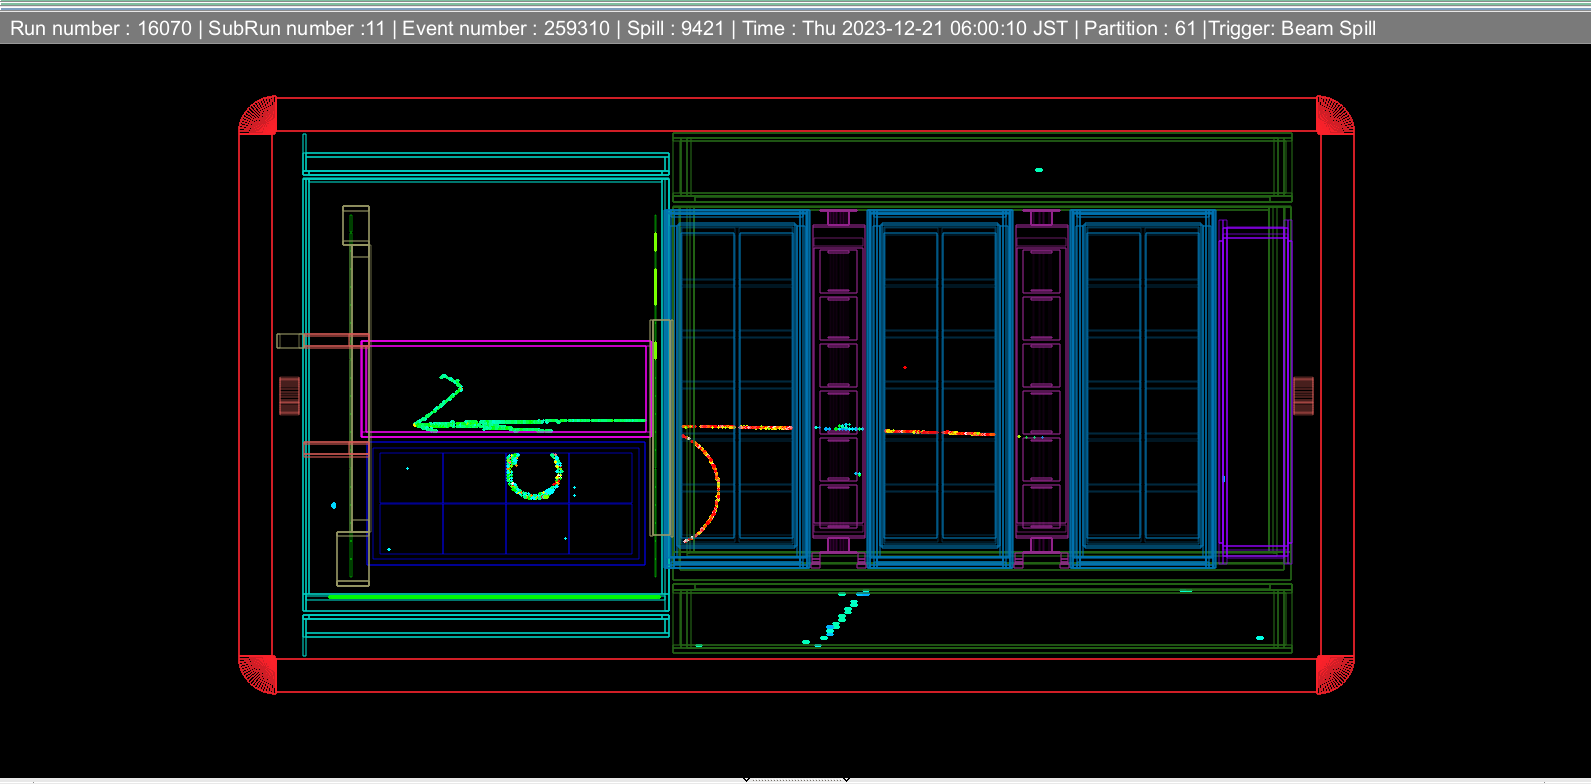
\includegraphics[width=0.5\linewidth]{fig/upgradeEvtDis.png}
        \caption{Event display of a possible $\pi^+$ event.}
        \label{fig:ndup-evedis}
    \end{figure}